\epigraph{Na egzaminie nie będzie przepływów, prawda?}{\textit{Student TCSu na dzień przed katastrofą}}
Zazwyczaj nie zajmuję się definiowaniem bo zakładam, że definicje są już znane, ale w przypadku sieci przepływowych zrobię wyjątek, bo na egzaminach pojawiają się pytania proszące o zdefiniowanie wszystkich pojęć z przepływów.

\textbf{Źródło} to wyróżniony wierzchołek, z którego krawędzie mogą jedynie ,,wychodzić'' (graf jest skierowany).

\textbf{Ujście} to wyróżniony wierzchołek, do którego krawędzie mogą jedynie ,,wchodzić''.

\textbf{$c$} jest to funkcja przepustowości, idąca ze zbioru krawędzi w liczby naturalne $>0$ (tak po ludzku to mówiona jaką przepustowość ma dana krawędź).

\textbf{Przepływem całkowitoliczbowym} nazywamy funkcję $f$ przyporządkowującą każdej krawędzi jakąś liczbę naturalną mniejszą lub równą jej przepustowości. Dla każdego wierzchołka który nie jest źródłem lub przepływem jest tak, że suma po funkcjach przepływów krawędzi do niego wchodzących jest równa sumie po funkcjach przepływów do niej wchodzących (co w sumie jest dosyć oczywiste, studenci zafiksowani na fizyce gadają tam o jakichś prawach kirchoffa i nie wiem o co im chodzi; studiuję TCS, nie prawo).

\textbf{Przekrojem} sieci przepływowej $S$ nazywamy jej ,,podział'' na 2 zbiory wierzchołków jej grafu $(S,T)$, taki, że: \begin{enumerate}
	\item $S \cup T = V$
	\item $S \cap T = \emptyset$
	\item Źródło jest w $S$
	\item Ujście jest w $T$
\end{enumerate}

\textbf{Przepustowością przekroju}, również oznaczaną przez $c$ (co generuje bałagan w oznaczeniach, ale to nie ja je wymyślałem) nazywamy sumę po przepustowościach wszystkich krawędzi wychodzących z $S$.

\textbf{Przepływem przez przekrój} nazywamy sumę po wartości funkcji $f$ dla wszystkich krawędzi które ,,wychodzą'' z $S$ pomniejszoną o sumę po wartości funkcji $f$ dla wszystkich krawędzi, które ,,wchodzą'' do $S$ (co jest dosyć intuicyjne, po prostu to co wypływa z $S$ minus to co wpływa).


\textbf{Przekrojem minimalnym} nazywamy przekrój o minimalnej przepustowości. Od razu można też zauważyć, że przepustowość sieci (w sensie to ile maksymalnie może wpłynąć do ujścia) jest mniejsza lub równa od przepustowości przekroju minimalnego. Dowodzi się to za pomocą dowodu \textit{to widać}. Formaliści mogą sobie nad tym podumać.

\textbf{Ścieżką powiększającą w przepływie} nazywamy zbiór krawędzi który będzie stanowić ścieżkę jeśli pominiemy ich skierowanie; generalnie to działa tak że musi ona iść od jakiegoś wierzchołka $v$ do innego wierzchołka $u$; zazwyczaj idzie ona od źródła do ujścia. Jeśli  dana krawędź idzie ,,do przodu'' to przepływ na niej nie może być równy przepustowości; jeśli idzie ,,do tyłu'' musi być niezerowy. Dlaczego to tak nazywamy? Bo jak do wszystkich krawędzi idących ,,do przodu'' dodamy 1 a od wszystkich idących ,,do tyłu'' odejmiemy 1 (a ścieżka szła od źródła do ujścia) to nadal mamy poprawny przepływ, w którym dodatku do ujścia wchodzi jedna jednostka więcej.

Przez $val(f)$ czasem będziemy oznaczać to, ile w danym przepływie wpływa do ujścia (i będziemy starali się maksymalizować tę wartość).

\begin{figure}[H]
	\centering
	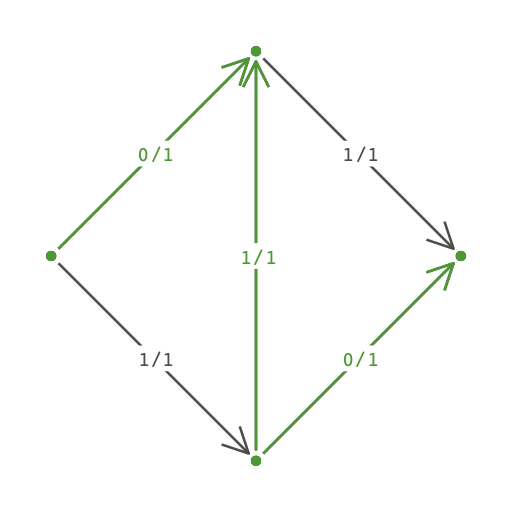
\includegraphics[scale=0.5]{images/augmenting_path.png}
	\caption{Przykład ścieżki powiększającej w sieci przepływowej}
\end{figure}
